\section{簡介}
本章節以及下一個章節將對於問答系統介紹,我們可將整個問答系統分成三個部分,首先針對使用者的查詢詞,透過檢索的方式回傳符合查詢詞的文本,但由於回傳的文本過多,因此我們需要一個過濾器(Filter)來判別此文本是否有此查詢詞之答案,以便降低文本的數量。最後在將這些被選出文本與其查詢詞,通過專注式記憶編碼解碼器(Attention-based Memory RNN Encoder-Decoder)抽取出可能的答案,進而回傳給使用者。本論文之研究的檢索部分是採用 Bing 搜尋來取得相關之文本,故僅針對過濾器以及專注式記憶編碼解碼器兩者進行詳細介紹。

在描述模型以前,我們將先簡介機器閱讀理解數據集。 Microsoft 釋出了閱讀理解相關的數據集,而以問答系統來實踐閱讀理解的概念。此數據集約莫有 10 萬筆的問答句以及約 20 萬以上的文章數,對於每個問句,都會有標註此問句的種類,如: cost to get a patent 是被分類為數值(Numeric)、 was ronald reagan a democrat 則是歸類成描述(Description)等等共 5 類。而 Bing 搜尋針對此問句,會提供大約 8 個左右的文本段落(Passages),人們再根據這些段落,標註此段落「是否」足夠提供問句之答案,並根據段落給予對應一至多個對應的答案。

\section{模型介紹}
\subsection{專注式記憶編碼解碼器}
圖 \ref{fig:dmn} 為本章節之系統架構圖之一。
\begin{figure}
    \centering
    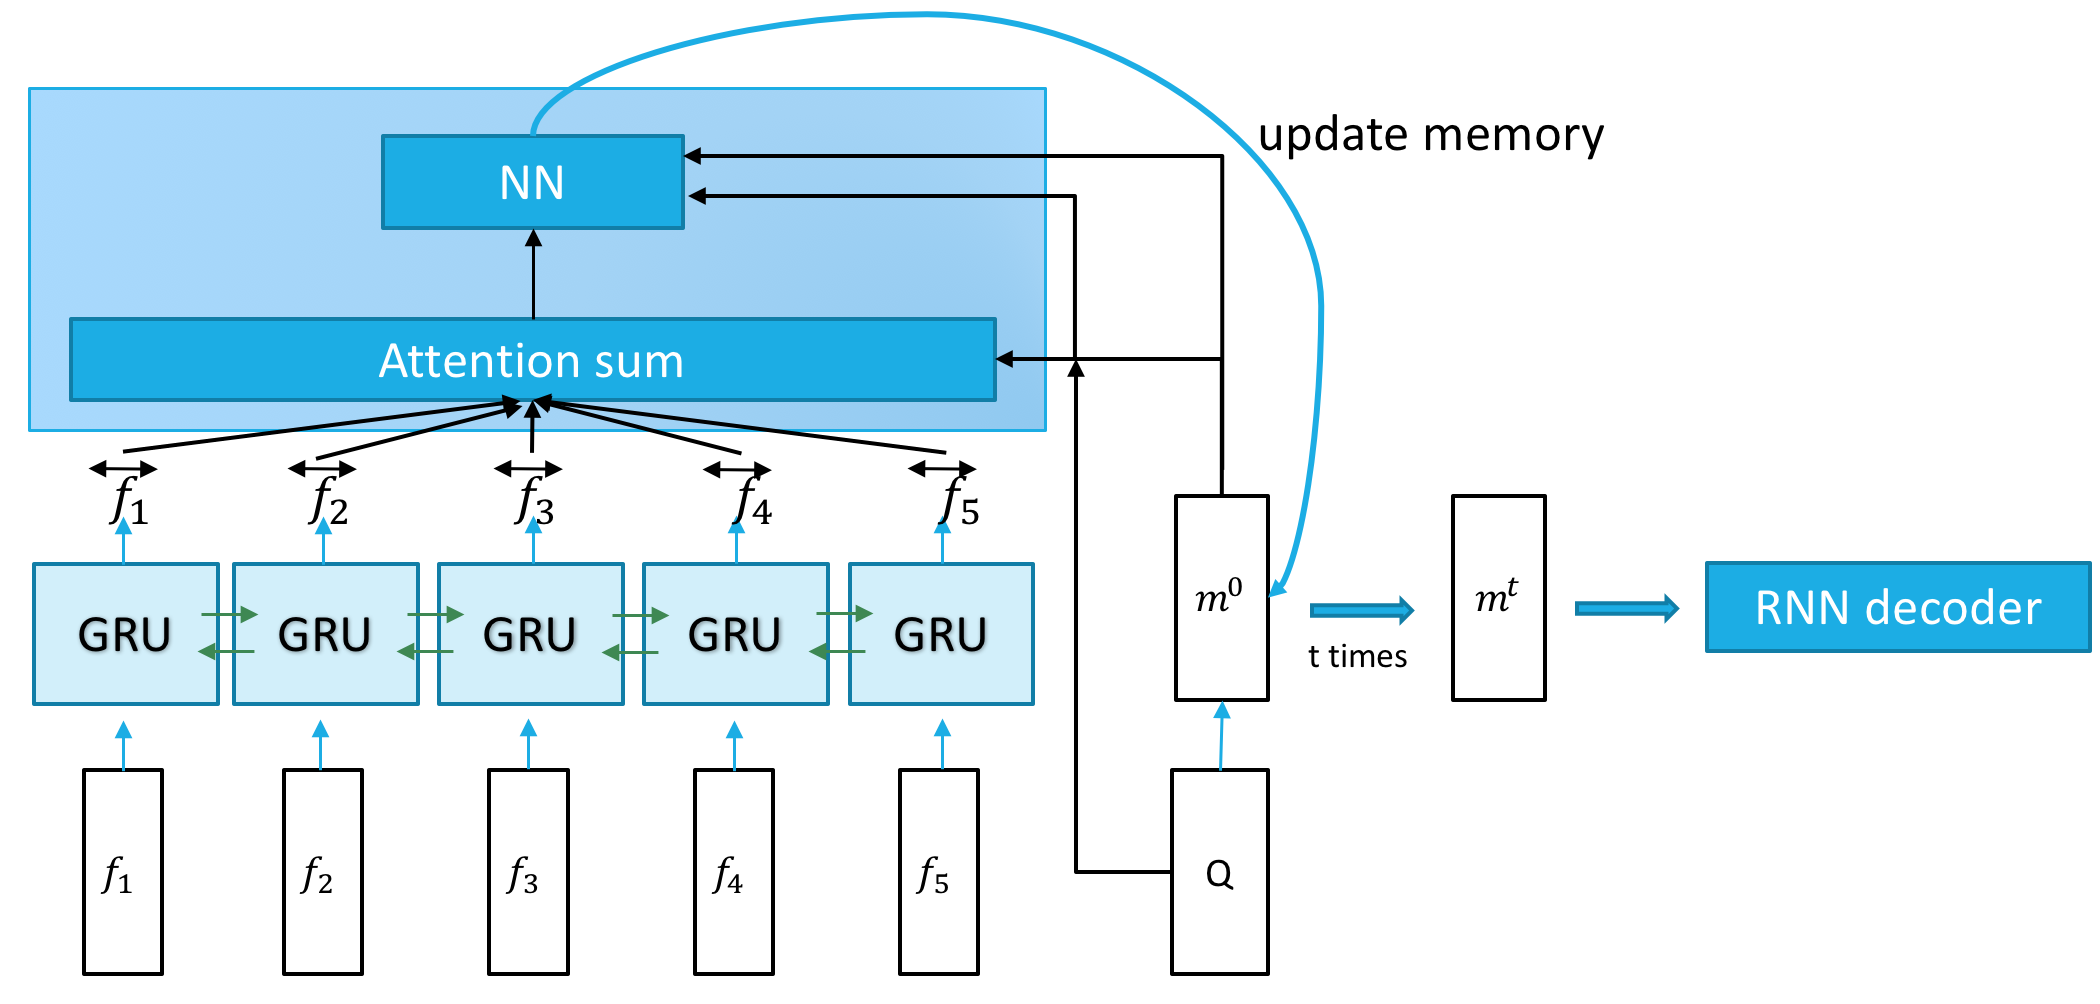
\includegraphics[scale=0.54]{images/chap3_dmn.png}
    \caption{專注式記憶編碼解碼器}\label{fig:dmn}
\end{figure}
%\subsubsection{模型介紹}
\begin{table}
    \caption{問句包含詞比例}
    \label{table:query_percentage}
    \centering
    \begin{tabular}[h]{|l|l|}
        \hline
        問句包含詞  &百分比\\
        \hline
        what        &42.2\%\\
        \hline
        how         &15.3\%\\
        \hline
        where       &4.4\%\\
        \hline
        when        &2.0\%\\
        \hline
        why         &1.8\%\\
        \hline
        who         &1.7\%\\
        \hline
        which       &1.4\%\\
        \hline
    \end{tabular}
\end{table}
\begin{table}
    \caption{答案種類}
    \label{table:query_type}
    \centering
    \begin{tabular}{|l|l|}
        \hline
        問句類型            &百分比\\
        \hline
        描述(Description) &52.6\%\\
        \hline
        數字(Numberic)    &28.4\%\\
        \hline
        名詞(Entity)      &10.5\%\\
        \hline
        地點(Location)    &5.7\%\\
        \hline
        人物(Person)      &2.7\%\\
        \hline
    \end{tabular}
\end{table}

